\documentclass[twoside]{book}

% Packages required by doxygen
\usepackage{calc}
\usepackage{doxygen}
\usepackage{graphicx}
\usepackage[utf8]{inputenc}
\usepackage{makeidx}
\usepackage{multicol}
\usepackage{multirow}
\usepackage{textcomp}
\usepackage[table]{xcolor}

% Font selection
\usepackage[T1]{fontenc}
\usepackage{mathptmx}
\usepackage[scaled=.90]{helvet}
\usepackage{courier}
\usepackage{amssymb}
\usepackage{sectsty}
\renewcommand{\familydefault}{\sfdefault}
\allsectionsfont{%
  \fontseries{bc}\selectfont%
  \color{darkgray}%
}
\renewcommand{\DoxyLabelFont}{%
  \fontseries{bc}\selectfont%
  \color{darkgray}%
}

% Page & text layout
\usepackage{geometry}
\geometry{%
  a4paper,%
  top=2.5cm,%
  bottom=2.5cm,%
  left=2.5cm,%
  right=2.5cm%
}
\tolerance=750
\hfuzz=15pt
\hbadness=750
\setlength{\emergencystretch}{15pt}
\setlength{\parindent}{0cm}
\setlength{\parskip}{0.2cm}
\makeatletter
\renewcommand{\paragraph}{%
  \@startsection{paragraph}{4}{0ex}{-1.0ex}{1.0ex}{%
    \normalfont\normalsize\bfseries\SS@parafont%
  }%
}
\renewcommand{\subparagraph}{%
  \@startsection{subparagraph}{5}{0ex}{-1.0ex}{1.0ex}{%
    \normalfont\normalsize\bfseries\SS@subparafont%
  }%
}
\makeatother

% Headers & footers
\usepackage{fancyhdr}
\pagestyle{fancyplain}
\fancyhead[LE]{\fancyplain{}{\bfseries\thepage}}
\fancyhead[CE]{\fancyplain{}{}}
\fancyhead[RE]{\fancyplain{}{\bfseries\leftmark}}
\fancyhead[LO]{\fancyplain{}{\bfseries\rightmark}}
\fancyhead[CO]{\fancyplain{}{}}
\fancyhead[RO]{\fancyplain{}{\bfseries\thepage}}
\fancyfoot[LE]{\fancyplain{}{}}
\fancyfoot[CE]{\fancyplain{}{}}
\fancyfoot[RE]{\fancyplain{}{\bfseries\scriptsize Generated on Wed Dec 18 2013 23\-:40\-:08 for My Project by Doxygen }}
\fancyfoot[LO]{\fancyplain{}{\bfseries\scriptsize Generated on Wed Dec 18 2013 23\-:40\-:08 for My Project by Doxygen }}
\fancyfoot[CO]{\fancyplain{}{}}
\fancyfoot[RO]{\fancyplain{}{}}
\renewcommand{\footrulewidth}{0.4pt}
\renewcommand{\chaptermark}[1]{%
  \markboth{#1}{}%
}
\renewcommand{\sectionmark}[1]{%
  \markright{\thesection\ #1}%
}

% Indices & bibliography
\usepackage{natbib}
\usepackage[titles]{tocloft}
\setcounter{tocdepth}{3}
\setcounter{secnumdepth}{5}
\makeindex

% Hyperlinks (required, but should be loaded last)
\usepackage{ifpdf}
\ifpdf
  \usepackage[pdftex,pagebackref=true]{hyperref}
\else
  \usepackage[ps2pdf,pagebackref=true]{hyperref}
\fi
\hypersetup{%
  colorlinks=true,%
  linkcolor=blue,%
  citecolor=blue,%
  unicode%
}

% Custom commands
\newcommand{\clearemptydoublepage}{%
  \newpage{\pagestyle{empty}\cleardoublepage}%
}


%===== C O N T E N T S =====

\begin{document}

% Titlepage & ToC
\hypersetup{pageanchor=false}
\pagenumbering{roman}
\begin{titlepage}
\vspace*{7cm}
\begin{center}%
{\Large My Project }\\
\vspace*{1cm}
{\large Generated by Doxygen 1.8.5}\\
\vspace*{0.5cm}
{\small Wed Dec 18 2013 23:40:08}\\
\end{center}
\end{titlepage}
\clearemptydoublepage
\tableofcontents
\clearemptydoublepage
\pagenumbering{arabic}
\hypersetup{pageanchor=true}

%--- Begin generated contents ---
\chapter{Hierarchical Index}
\section{Class Hierarchy}
This inheritance list is sorted roughly, but not completely, alphabetically\-:\begin{DoxyCompactList}
\item \contentsline{section}{com.\-android.\-server.\-power.\-Display\-Power\-Controller.\-Callbacks}{\pageref{interfacecom_1_1android_1_1server_1_1power_1_1DisplayPowerController_1_1Callbacks}}{}
\item Death\-Recipient\begin{DoxyCompactList}
\item \contentsline{section}{com.\-android.\-server.\-power.\-Power\-Manager\-Service.\-Htc\-Cpu\-Ctrl}{\pageref{classcom_1_1android_1_1server_1_1power_1_1PowerManagerService_1_1HtcCpuCtrl}}{}
\item \contentsline{section}{com.\-android.\-server.\-power.\-Power\-Manager\-Service.\-Wake\-Lock}{\pageref{classcom_1_1android_1_1server_1_1power_1_1PowerManagerService_1_1WakeLock}}{}
\end{DoxyCompactList}
\item \contentsline{section}{com.\-android.\-server.\-power.\-Power\-Manager\-Service.\-Display\-Blanker\-Impl}{\pageref{classcom_1_1android_1_1server_1_1power_1_1PowerManagerService_1_1DisplayBlankerImpl}}{}
\item \contentsline{section}{com.\-android.\-server.\-power.\-Display\-Power\-Controller.\-D\-P\-C\-Internal\-A\-P\-I}{\pageref{classcom_1_1android_1_1server_1_1power_1_1DisplayPowerController_1_1DPCInternalAPI}}{}
\item Monitor\begin{DoxyCompactList}
\item \contentsline{section}{com.\-android.\-server.\-power.\-Power\-Manager\-Service}{\pageref{classcom_1_1android_1_1server_1_1power_1_1PowerManagerService}}{}
\end{DoxyCompactList}
\item On\-Dismiss\-Listener\begin{DoxyCompactList}
\item \contentsline{section}{com.\-android.\-server.\-power.\-Shutdown\-Thread.\-Close\-Dialog\-Receiver}{\pageref{classcom_1_1android_1_1server_1_1power_1_1ShutdownThread_1_1CloseDialogReceiver}}{}
\end{DoxyCompactList}
\item \contentsline{section}{com.\-android.\-server.\-power.\-Display\-Power\-State.\-Photonic\-Modulator}{\pageref{classcom_1_1android_1_1server_1_1power_1_1DisplayPowerState_1_1PhotonicModulator}}{}
\item \contentsline{section}{com.\-android.\-server.\-power.\-Power\-Manager\-Service.\-P\-M\-S\-Internal\-A\-P\-I}{\pageref{classcom_1_1android_1_1server_1_1power_1_1PowerManagerService_1_1PMSInternalAPI}}{}
\item \contentsline{section}{com.\-android.\-server.\-power.\-Power\-Manager\-Service.\-Screen\-On\-Blocker\-Impl}{\pageref{classcom_1_1android_1_1server_1_1power_1_1PowerManagerService_1_1ScreenOnBlockerImpl}}{}
\item Stub\begin{DoxyCompactList}
\item \contentsline{section}{com.\-android.\-server.\-power.\-Power\-Manager\-Service}{\pageref{classcom_1_1android_1_1server_1_1power_1_1PowerManagerService}}{}
\end{DoxyCompactList}
\item \contentsline{section}{com.\-android.\-server.\-power.\-Power\-Manager\-Service.\-Suspend\-Blocker\-Impl}{\pageref{classcom_1_1android_1_1server_1_1power_1_1PowerManagerService_1_1SuspendBlockerImpl}}{}
\item Thread\begin{DoxyCompactList}
\item \contentsline{section}{com.\-android.\-server.\-power.\-Shutdown\-Thread}{\pageref{classcom_1_1android_1_1server_1_1power_1_1ShutdownThread}}{}
\end{DoxyCompactList}
\item Broadcast\-Receiver\begin{DoxyCompactList}
\item \contentsline{section}{com.\-android.\-server.\-power.\-Power\-Manager\-Service.\-Battery\-Receiver}{\pageref{classcom_1_1android_1_1server_1_1power_1_1PowerManagerService_1_1BatteryReceiver}}{}
\item \contentsline{section}{com.\-android.\-server.\-power.\-Power\-Manager\-Service.\-Boot\-Completed\-Receiver}{\pageref{classcom_1_1android_1_1server_1_1power_1_1PowerManagerService_1_1BootCompletedReceiver}}{}
\item \contentsline{section}{com.\-android.\-server.\-power.\-Power\-Manager\-Service.\-Dock\-Receiver}{\pageref{classcom_1_1android_1_1server_1_1power_1_1PowerManagerService_1_1DockReceiver}}{}
\item \contentsline{section}{com.\-android.\-server.\-power.\-Power\-Manager\-Service.\-Dream\-Receiver}{\pageref{classcom_1_1android_1_1server_1_1power_1_1PowerManagerService_1_1DreamReceiver}}{}
\item \contentsline{section}{com.\-android.\-server.\-power.\-Power\-Manager\-Service.\-O\-O\-B\-E\-Timeout\-Receiver}{\pageref{classcom_1_1android_1_1server_1_1power_1_1PowerManagerService_1_1OOBETimeoutReceiver}}{}
\item \contentsline{section}{com.\-android.\-server.\-power.\-Power\-Manager\-Service.\-User\-Switched\-Receiver}{\pageref{classcom_1_1android_1_1server_1_1power_1_1PowerManagerService_1_1UserSwitchedReceiver}}{}
\item \contentsline{section}{com.\-android.\-server.\-power.\-Shutdown\-Thread.\-Close\-Dialog\-Receiver}{\pageref{classcom_1_1android_1_1server_1_1power_1_1ShutdownThread_1_1CloseDialogReceiver}}{}
\end{DoxyCompactList}
\item Content\-Observer\begin{DoxyCompactList}
\item \contentsline{section}{com.\-android.\-server.\-power.\-Power\-Manager\-Service.\-Settings\-Observer}{\pageref{classcom_1_1android_1_1server_1_1power_1_1PowerManagerService_1_1SettingsObserver}}{}
\end{DoxyCompactList}
\item Display\-Transaction\-Listener\begin{DoxyCompactList}
\item \contentsline{section}{com.\-android.\-server.\-power.\-Electron\-Beam.\-Natural\-Surface\-Layout}{\pageref{classcom_1_1android_1_1server_1_1power_1_1ElectronBeam_1_1NaturalSurfaceLayout}}{}
\end{DoxyCompactList}
\item Handler\begin{DoxyCompactList}
\item \contentsline{section}{com.\-android.\-server.\-power.\-Display\-Power\-Controller.\-Display\-Controller\-Handler}{\pageref{classcom_1_1android_1_1server_1_1power_1_1DisplayPowerController_1_1DisplayControllerHandler}}{}
\item \contentsline{section}{com.\-android.\-server.\-power.\-Notifier.\-Notifier\-Handler}{\pageref{classcom_1_1android_1_1server_1_1power_1_1Notifier_1_1NotifierHandler}}{}
\item \contentsline{section}{com.\-android.\-server.\-power.\-Power\-Manager\-Service.\-Power\-Manager\-Handler}{\pageref{classcom_1_1android_1_1server_1_1power_1_1PowerManagerService_1_1PowerManagerHandler}}{}
\end{DoxyCompactList}
\end{DoxyCompactList}

\chapter{Class Index}
\section{Class List}
Here are the classes, structs, unions and interfaces with brief descriptions\-:\begin{DoxyCompactList}
\item\contentsline{section}{\hyperlink{classAnimal}{Animal} }{\pageref{classAnimal}}{}
\item\contentsline{section}{\hyperlink{classCat}{Cat} }{\pageref{classCat}}{}
\item\contentsline{section}{\hyperlink{classDog}{Dog} }{\pageref{classDog}}{}
\end{DoxyCompactList}

\chapter{File Index}
\section{File List}
Here is a list of all files with brief descriptions\-:\begin{DoxyCompactList}
\item\contentsline{section}{\hyperlink{DisplayBlanker_8java}{Display\-Blanker.\-java} }{\pageref{DisplayBlanker_8java}}{}
\item\contentsline{section}{\hyperlink{DisplayPowerController_8java}{Display\-Power\-Controller.\-java} }{\pageref{DisplayPowerController_8java}}{}
\item\contentsline{section}{\hyperlink{DisplayPowerRequest_8java}{Display\-Power\-Request.\-java} }{\pageref{DisplayPowerRequest_8java}}{}
\item\contentsline{section}{\hyperlink{DisplayPowerState_8java}{Display\-Power\-State.\-java} }{\pageref{DisplayPowerState_8java}}{}
\item\contentsline{section}{\hyperlink{ElectronBeam_8java}{Electron\-Beam.\-java} }{\pageref{ElectronBeam_8java}}{}
\item\contentsline{section}{\hyperlink{Notifier_8java}{Notifier.\-java} }{\pageref{Notifier_8java}}{}
\item\contentsline{section}{\hyperlink{PowerManagerService_8java}{Power\-Manager\-Service.\-java} }{\pageref{PowerManagerService_8java}}{}
\item\contentsline{section}{\hyperlink{RampAnimator_8java}{Ramp\-Animator.\-java} }{\pageref{RampAnimator_8java}}{}
\item\contentsline{section}{\hyperlink{ScreenOnBlocker_8java}{Screen\-On\-Blocker.\-java} }{\pageref{ScreenOnBlocker_8java}}{}
\item\contentsline{section}{\hyperlink{ShutdownThread_8java}{Shutdown\-Thread.\-java} }{\pageref{ShutdownThread_8java}}{}
\item\contentsline{section}{\hyperlink{SuspendBlocker_8java}{Suspend\-Blocker.\-java} }{\pageref{SuspendBlocker_8java}}{}
\item\contentsline{section}{\hyperlink{WirelessChargerDetector_8java}{Wireless\-Charger\-Detector.\-java} }{\pageref{WirelessChargerDetector_8java}}{}
\end{DoxyCompactList}

\chapter{Class Documentation}
\hypertarget{classAnimal}{\section{Animal Class Reference}
\label{classAnimal}\index{Animal@{Animal}}
}


Inheritance diagram for Animal\-:
\nopagebreak
\begin{figure}[H]
\begin{center}
\leavevmode
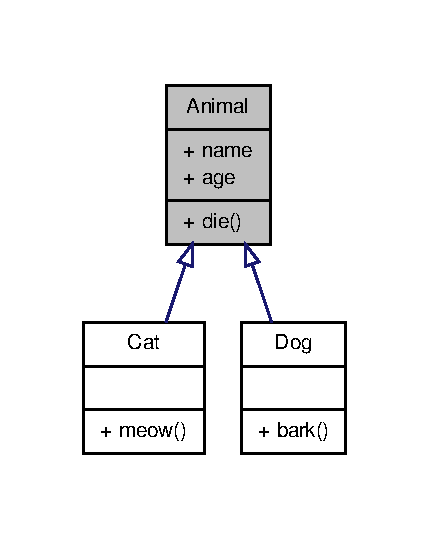
\includegraphics[width=206pt]{classAnimal__inherit__graph}
\end{center}
\end{figure}


Collaboration diagram for Animal\-:
\nopagebreak
\begin{figure}[H]
\begin{center}
\leavevmode
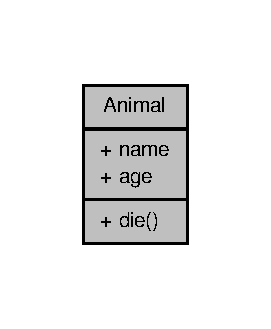
\includegraphics[width=130pt]{classAnimal__coll__graph}
\end{center}
\end{figure}
\subsection*{Public Member Functions}
\begin{DoxyCompactItemize}
\item 
void \hyperlink{classAnimal_a557fe0d71dda75be2f8459ce0d7c2275}{die} ()
\end{DoxyCompactItemize}
\subsection*{Public Attributes}
\begin{DoxyCompactItemize}
\item 
string \hyperlink{classAnimal_a9cf3bfd9070daec7b3bbc87cbd958f35}{name}
\item 
int \hyperlink{classAnimal_a31e4a23bef9596927496de4eb6b9c721}{age}
\end{DoxyCompactItemize}


\subsection{Member Function Documentation}
\hypertarget{classAnimal_a557fe0d71dda75be2f8459ce0d7c2275}{\index{Animal@{Animal}!die@{die}}
\index{die@{die}!Animal@{Animal}}
\subsubsection[{die}]{\setlength{\rightskip}{0pt plus 5cm}void Animal\-::die (
\begin{DoxyParamCaption}
{}
\end{DoxyParamCaption}
)}}\label{classAnimal_a557fe0d71dda75be2f8459ce0d7c2275}


\subsection{Member Data Documentation}
\hypertarget{classAnimal_a31e4a23bef9596927496de4eb6b9c721}{\index{Animal@{Animal}!age@{age}}
\index{age@{age}!Animal@{Animal}}
\subsubsection[{age}]{\setlength{\rightskip}{0pt plus 5cm}int Animal\-::age}}\label{classAnimal_a31e4a23bef9596927496de4eb6b9c721}
\hypertarget{classAnimal_a9cf3bfd9070daec7b3bbc87cbd958f35}{\index{Animal@{Animal}!name@{name}}
\index{name@{name}!Animal@{Animal}}
\subsubsection[{name}]{\setlength{\rightskip}{0pt plus 5cm}string Animal\-::name}}\label{classAnimal_a9cf3bfd9070daec7b3bbc87cbd958f35}


The documentation for this class was generated from the following file\-:\begin{DoxyCompactItemize}
\item 
\hyperlink{example_8cpp}{example.\-cpp}\end{DoxyCompactItemize}

\hypertarget{classCat}{\section{Cat Class Reference}
\label{classCat}\index{Cat@{Cat}}
}


Inheritance diagram for Cat\-:
\nopagebreak
\begin{figure}[H]
\begin{center}
\leavevmode
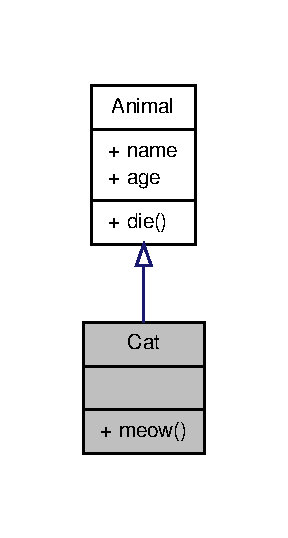
\includegraphics[width=138pt]{classCat__inherit__graph}
\end{center}
\end{figure}


Collaboration diagram for Cat\-:
\nopagebreak
\begin{figure}[H]
\begin{center}
\leavevmode
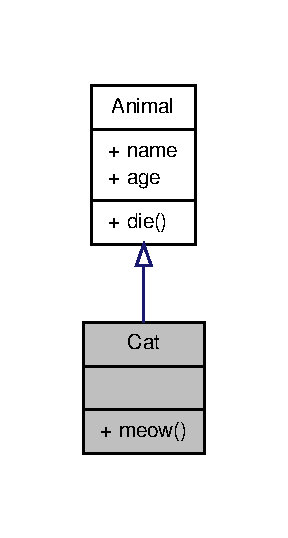
\includegraphics[width=138pt]{classCat__coll__graph}
\end{center}
\end{figure}
\subsection*{Public Member Functions}
\begin{DoxyCompactItemize}
\item 
void \hyperlink{classCat_aa770c672b7458b036d7384a6915d9367}{meow} ()
\end{DoxyCompactItemize}
\subsection*{Additional Inherited Members}


\subsection{Member Function Documentation}
\hypertarget{classCat_aa770c672b7458b036d7384a6915d9367}{\index{Cat@{Cat}!meow@{meow}}
\index{meow@{meow}!Cat@{Cat}}
\subsubsection[{meow}]{\setlength{\rightskip}{0pt plus 5cm}void Cat\-::meow (
\begin{DoxyParamCaption}
{}
\end{DoxyParamCaption}
)}}\label{classCat_aa770c672b7458b036d7384a6915d9367}


The documentation for this class was generated from the following file\-:\begin{DoxyCompactItemize}
\item 
\hyperlink{example_8cpp}{example.\-cpp}\end{DoxyCompactItemize}

\hypertarget{classDog}{\section{Dog Class Reference}
\label{classDog}\index{Dog@{Dog}}
}


Inheritance diagram for Dog\-:
\nopagebreak
\begin{figure}[H]
\begin{center}
\leavevmode
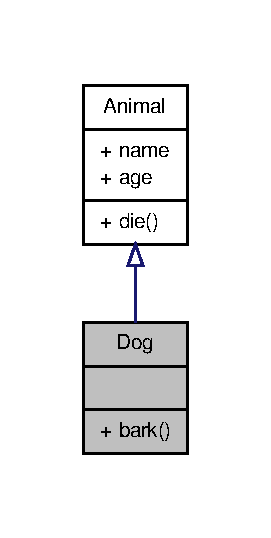
\includegraphics[width=130pt]{classDog__inherit__graph}
\end{center}
\end{figure}


Collaboration diagram for Dog\-:
\nopagebreak
\begin{figure}[H]
\begin{center}
\leavevmode
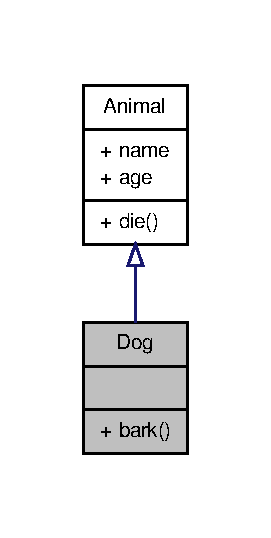
\includegraphics[width=130pt]{classDog__coll__graph}
\end{center}
\end{figure}
\subsection*{Public Member Functions}
\begin{DoxyCompactItemize}
\item 
void \hyperlink{classDog_ad3ab5661e3663948a486ff73049b1e1f}{bark} ()
\end{DoxyCompactItemize}
\subsection*{Additional Inherited Members}


\subsection{Member Function Documentation}
\hypertarget{classDog_ad3ab5661e3663948a486ff73049b1e1f}{\index{Dog@{Dog}!bark@{bark}}
\index{bark@{bark}!Dog@{Dog}}
\subsubsection[{bark}]{\setlength{\rightskip}{0pt plus 5cm}void Dog\-::bark (
\begin{DoxyParamCaption}
{}
\end{DoxyParamCaption}
)}}\label{classDog_ad3ab5661e3663948a486ff73049b1e1f}


The documentation for this class was generated from the following file\-:\begin{DoxyCompactItemize}
\item 
\hyperlink{example_8cpp}{example.\-cpp}\end{DoxyCompactItemize}

\chapter{File Documentation}
\hypertarget{example_8cpp}{\section{example.\-cpp File Reference}
\label{example_8cpp}\index{example.\-cpp@{example.\-cpp}}
}
\subsection*{Classes}
\begin{DoxyCompactItemize}
\item 
class \hyperlink{classAnimal}{Animal}
\item 
class \hyperlink{classDog}{Dog}
\item 
class \hyperlink{classCat}{Cat}
\end{DoxyCompactItemize}

%--- End generated contents ---

% Index
\newpage
\phantomsection
\addcontentsline{toc}{chapter}{Index}
\printindex

\end{document}
